\documentclass[../structural_economics_book.tex]{subfiles}
\begin{document}
\ifSubfilesClassLoaded{\setcounter{chapter}{3}}{}
\chapter{What the Standard Model Assumes}\label{ch:04}
\chaptersubtitle{Six Properties of One Matrix}
% TODO-VERIFY: this epigraph appears to follow a secondary-source paraphrase. The original (Sunkel and Paz 1970, Introduction) reads approximately "... el subdesarrollo no es un momento en la evolucion continua de una sociedad economica, politica y culturalmente aislada y autonoma ... el subdesarrollo es parte del proceso historico global de desarrollo ..."; "ni una 'etapa'" and "del capitalismo" may not be in the text. Check against the Siglo XXI 1970 edition and give the page; if it is a paraphrase, drop the quotation marks.
\begin{quote}
\textit{``El subdesarrollo no es un `momento' ni una `etapa' en la evoluci\'{o}n de una sociedad aislada y aut\'{o}noma, sino parte del proceso hist\'{o}rico global de desarrollo del capitalismo.''}\\[0.3em]
\textnormal{[``Underdevelopment is not a `moment' or a `stage' in the evolution of an isolated and autonomous society, but part of the global historical process of capitalist development.'']}\\
\hfill --- Osvaldo Sunkel and Pedro Paz, \textit{El subdesarrollo latinoamericano y la teor\'{i}a del desarrollo} (1970)
\end{quote}

\vspace{1em}

The first three chapters rewrote the standard model in matrix notation. Chapter~1 showed that anonymous, price-mediated interaction implies $W^{\text{mkt}} = \ones\mathbf{s}'$, and named its equal-endowment case $W^{CE} = \frac{1}{N}\ones\ones'$. Chapter~2 showed which departures from it break efficiency ($W^U \neq 0$) and which are distributional (unequal $\boldsymbol{\pi}$). Chapter~3 showed that growth propagation depends on the production structure $A$.

This chapter pulls the threads together. It catalogs, in one place, the assumptions from which the benchmark model abstracts --- six properties, most of them properties of one matrix --- and for each assumption states: (a) the formal condition, (b) when it approximately holds, (c) when it fails, (d) what the world looks like when it does, and (e) which chapter in this book develops the general case.

This is the hinge. Part~I ends here. Part~II begins with $W$ as an object to be studied rather than assumed.


%% =====================================================================
\section{The Six Assumptions}
\label{ch04:sec:six}
%% =====================================================================

Recall from Chapter~1 that the competitive benchmark $W^{CE} = \frac{1}{N}\ones\ones'$ has five properties: doubly stochastic, symmetric, rank~1, equal power, unit spectral gap. The benchmark Arrow--Debreu model abstracts from several kinds of structure; the six assumptions below make that abstraction explicit. The sixth is not a property of any matrix but of the model that uses it: preferences are exogenous.

\begin{definition}[The Six Assumptions of the Standard Model]\label{ch04:def:six}
The benchmark competitive model abstracts from the following (``assumes'' in what follows means ``is built so that''):
\begin{enumerate}
\item[\textbf{A1.}] \textbf{No utility externalities.} $W^U = 0$ (or equivalently $\gamma_U = 0$). Agent $i$'s utility depends only on $x_i$.
\item[\textbf{A2.}] \textbf{Exogenous production structure.} The technical coefficients $A$ (and hence $W^P = D^{-1}A$) are taken as given from input-output data: a technological fact, not a social choice.
\item[\textbf{A3.}] \textbf{No information network.} Beliefs are not formed through social channels: there is no $W^I$ along which one agent's beliefs move another's.
\item[\textbf{A4.}] \textbf{Anonymous market interaction.} The price mechanism aggregates demands anonymously, weighting agents by wealth shares: $W^{\text{mkt}} = \ones\mathbf{s}'$ (Chapter~1, Definition~\ref{ch01:def:market_W}).
\item[\textbf{A5.}] \textbf{Equal power.} The left Perron vector of the composite interaction matrix is $\boldsymbol{\pi} = \frac{1}{N}\ones$. No agent has more structural influence than any other. In the benchmark this holds only with equal endowments, since $\boldsymbol{\pi}(W^{\text{mkt}}) = \mathbf{s}$.
\item[\textbf{A6.}] \textbf{Exogenous preferences.} $\theta_i$ (the preference parameter governing patience, risk aversion, time discount, labor supply) is fixed. It does not evolve in response to the network.
\end{enumerate}
\end{definition}

We now examine each assumption in detail.


%% =====================================================================
\section{A1: No Utility Externalities ($W^U = 0$)}
\label{ch04:sec:A1}
%% =====================================================================

\subsection{The Formal Condition}

Agent $i$ maximizes $U_i(x_i)$, not $V_i(\x) = U_i(x_i) + \gamma_U \sum_j W^U_{ij} U_j(x_j)$. Nobody's consumption enters anyone else's utility function. No altruism, no envy, no status competition, no compadrazgo bonds, no peer effects.

\subsection{When It Approximately Holds}

Large anonymous markets for standardized goods. The buyer of a barrel of oil on the NYMEX does not care who produced it. The seller of wheat at the Chicago Board of Trade does not know who will eat it. In these settings, the externality weights $W^U_{ij}$ are effectively zero because the transacting parties have no social relationship.

\subsection{When It Fails}

\textbf{Small communities.} In a village or a tight-knit neighborhood, people know each other. The api vendor cares about her comadre's income. The shopkeeper cares about the schoolteacher's welfare. Utility externalities are large, local, and asymmetric.

\textbf{Status competition.} Veblen (1899), Duesenberry (1949), Frank (1985): consumption generates externalities through social comparison. A neighbor's new car reduces your satisfaction with your old one. The externality is negative and proportional to the visibility of consumption.

\textbf{Network effects.} Adoption of a technology by agent $j$ raises the value of the technology for agent $i$ (telephones, social media, payment systems). $W^U_{ij} > 0$ for complementary users.

\begin{proposition}[Welfare Cost of Ignoring $W^U$]\label{ch04:prop:A1_cost}
In the one-good quadratic economy of Chapter~2, when $W^U \neq 0$ and $\gamma_U > 0$, the externality-blind allocation (which ignores $W^U$) generates a social-welfare loss of
\begin{equation}\label{ch04:eq:A1_loss}
L_{A1} = \gamma_U^2 \cdot \Var(c_j^U) \cdot \Psi,
\end{equation}
where $c_j^U = \sum_{i \neq j} W^U_{ij}$ is agent $j$'s externality centrality in the utility network, to second order in $\gamma_U$, with $\Psi = N(1-\kappa m)^2/(2\kappa)$ in the quadratic economy (Chapter~2, Proposition~\ref{ch02:prop:ext_loss}, which also gives the exact formula).
\end{proposition}

\textbf{Relaxed in:} Chapters~5 (the utility network defined), 7 (bargaining equilibrium with externalities), 12 (welfare under endogenous preferences).


%% =====================================================================
\section{A2: Exogenous Production Structure ($W^P$ Given)}
\label{ch04:sec:A2}
%% =====================================================================

\subsection{The Formal Condition}

The technical coefficients matrix $A$ is treated as a technological parameter: determined by engineering, not by economic choices. The Leontief system takes $A$ as data and solves for output given final demand. This is a feature of the fixed-coefficient benchmark, not of general-equilibrium theory as such: with Cobb-Douglas or CES technologies, input shares respond to prices, and recent work makes the network itself endogenous (Oberfield 2018; Acemoglu and Azar 2020). What such work rarely does is treat $A$ as an object of development policy.

\subsection{When It Approximately Holds}

Short-run analysis. In a given year, a steel plant requires a specific amount of iron ore, coal, and electricity per ton of steel. These technical coefficients change slowly. For short-run comparative statics, treating $A$ as fixed is reasonable.

\subsection{When It Fails}

\textbf{ISI as structural policy.} The entire history of import-substitution industrialization is an attempt to \textit{change} $A$ --- to build domestic production of goods previously imported. Tavares (1972) documented how each external bottleneck provoked a structural response that altered the domestic input-output matrix. $A$ is a policy variable, not a constant.

\textbf{Endogenous specialization.} Countries choose what to produce. The product space (Hidalgo et al., 2007) shows that diversification follows path-dependent trajectories shaped by the existing productive structure: a country that produces wine can more easily diversify into grapes, bottles, and corks than into semiconductors. The production network evolves.

\textbf{FDI and global value chains.} When a multinational opens an assembly plant, it inserts new rows and columns into the domestic $A$, connecting the domestic economy to the global production network. The entries of $A$ reflect corporate decisions, not just technology.

\begin{proposition}[Endogenous $W^P$ Changes the Growth Trajectory]\label{ch04:prop:A2_growth}
In the multi-sector growth model of Chapter~3, write $L_\gamma = (I - \gamma A')^{-1}$ and $F' = \text{diag}(\partial f_i/\partial K_i)$ at the steady state $\K^*$. If $\Delta - SL_\gamma F'$ is invertible, a small change $\Delta A$ in the technical coefficients shifts the steady-state capital vector by
\begin{equation}
\Delta \K^* \approx \bigl(\Delta - S L_\gamma F'\bigr)^{-1} S\, L_\gamma\,(\gamma\,\Delta A')\,L_\gamma\, \mathbf{f}(\K^*).
\end{equation}
The effect is amplified by the Leontief inverse \textit{twice} --- once for the direct impact, once for the propagation through the existing network --- and then by the steady-state feedback $(\Delta - SL_\gamma F')^{-1}$. A small change in $A$ can have a large effect on $\K^*$ if the Leontief inverse has large off-diagonal entries.
\end{proposition}

\begin{proof}
The steady state satisfies $\Delta\K^* = S L_\gamma \mathbf{f}(\K^*)$. Differentiate: $\Delta\, d\K = S\,(dL_\gamma)\,\mathbf{f} + S L_\gamma F' d\K$, and $dL_\gamma = L_\gamma(\gamma\, dA')L_\gamma$ (differentiate $L_\gamma(I - \gamma A') = I$). Solve for $d\K$. (For the two-sector economy of Chapter~3, Example~\ref{ch03:ex:two_WP}, raising $a_{12}$ by $0.01$ moves $\K^*$ by $(0.089, 0.269)$ by this formula and by $(0.089, 0.270)$ by direct computation; \texttt{code/ch04.py}.)
\end{proof}

\textbf{Relaxed in:} Chapters~3 (production network in growth), 13 (how networks evolve), 15 (operator design --- policy as deliberate change of $W^P$).


%% =====================================================================
\section{A3: No Information Network ($W^I$ Absent)}
\label{ch04:sec:A3}
%% =====================================================================

\subsection{The Formal Condition}

The benchmark Arrow--Debreu model abstracts from belief formation through social networks: agents know the relevant prices and probabilities, and there is no mechanism through which one agent's beliefs influence another's --- no $W^I$. Mainstream economics relaxes much of this, with asymmetric information and with Bayesian learning in social networks (Acemoglu, Dahleh, Lobel and Ozdaglar 2011). What it rarely does is make the weights $W^I$ themselves the object of study.

\subsection{When It Approximately Holds}

Financial markets with mandatory disclosure, standardized goods with transparent pricing, and repeated interactions where agents learn the true model. In these settings, heterogeneous beliefs converge to the truth through Bayesian updating, making $W^I$ unimportant.

\subsection{When It Fails}

\textbf{DeGroot-style learning.} Agents in many real-world settings do not observe the data-generating process. They observe their neighbors' behavior, their social media feeds, their peers' outcomes. There is experimental evidence that, in some settings, people update closer to a weighted average of neighbors' beliefs than to the Bayesian benchmark (Chandrasekhar, Larreguy and Xandri 2020). Under such averaging the long-run consensus weights are the Perron vector of $W^I$ (DeGroot 1974): the agents with the most epistemic power determine the consensus, whether or not their initial beliefs are correct. Golub and Jackson (2010) characterize when the consensus is nevertheless correct in large networks (the ``wisdom of crowds'').

\textbf{Media concentration.} When a few outlets control information flow, $W^I$ is star-shaped: everyone listens to the hub. The consensus converges to the hub's beliefs. State media, monopoly platforms, and algorithmic feeds all produce this topology.

\textbf{Aspiration formation.} The girl in Potos\'{i} does not observe the ``true'' return to education. She observes the returns \textit{in her network} --- her mother, her school friends, her cousin in Buenos Aires, her TikTok feed. Her perceived returns are $W^I$-weighted averages of the returns experienced by her reference group. This shapes her aspirations, her investment in education, and ultimately her economic outcomes.

\begin{proposition}[Epistemic Power and Belief Convergence]\label{ch04:prop:A3_beliefs}
Under DeGroot learning on an information network $W^I$ (row-stochastic, irreducible, aperiodic):
\begin{equation}
\lim_{t \to \infty} \mathbf{b}^{(t)} = (\boldsymbol{\pi}^I)' \mathbf{b}^{(0)} \cdot \ones,
\end{equation}
where $\boldsymbol{\pi}^I$ is the left Perron eigenvector of $W^I$. The long-run consensus is a weighted average of initial beliefs, with weights given by epistemic power $\pi^I_j$. Agents with $\pi^I_j \gg 1/N$ dominate the consensus.
\end{proposition}

\begin{proof}
$\mathbf{b}^{(t)} = (W^I)^t\mathbf{b}^{(0)}$. For a primitive (irreducible and aperiodic) stochastic matrix, $(W^I)^t \to \ones(\boldsymbol{\pi}^I)'$ by Perron--Frobenius (Chapter~6).
\end{proof}

\textbf{Relaxed in:} Chapters~5 (the information network defined), 8 (belief manipulation and epistemic power), 9--12 (the formation model, where $W^I$ shapes preferences).


%% =====================================================================
\section{A4: Anonymous Market Interaction (\texorpdfstring{$W^{\text{mkt}} = \ones\mathbf{s}'$}{W\textasciicircum mkt = 1s'})}
\label{ch04:sec:A4}
%% =====================================================================

\subsection{The Formal Condition}

The competitive price mechanism aggregates demands anonymously. Each agent's weight in aggregate demand is her expenditure share $s_i$ ($1/N$ with equal budgets). Nobody has market power. The interaction is $W^{\text{mkt}} = \ones\mathbf{s}'$, which is $W^{CE}$ under equal endowments (Chapter~1, Section~\ref{ch01:sec:implicit_W}).

\subsection{When It Approximately Holds}

Markets with many small agents, homogeneous goods, free entry and exit, and complete information. The textbook examples: wheat markets, foreign exchange (at the retail level), standardized commodity markets with many participants.

\subsection{When It Fails}

\textbf{Monopsony and monopoly.} A single buyer (monopsony employer in a company town) or single seller (a state monopoly in domestic gas distribution) sets prices rather than taking them. The interaction matrix has a star topology: $W_{ij}^{\text{mkt}} \approx 0$ for all $j$ except the hub.

\textbf{Platform economies.} Amazon, Uber, and Airbnb are hubs through which millions of small agents must transact. The platform sets the terms of trade. $W^{\text{mkt}}$ is star-shaped with the platform at the center.

\textbf{Bargaining.} In thin markets (few participants, differentiated goods, relationship-specific investments), prices are determined by bilateral bargaining rather than anonymous market clearing. The allocation depends on relative bargaining power, which is a function of the network position (Chapter~7).

\begin{proposition}[Distributional Loss from Market Power]\label{ch04:prop:A4_loss}
When interaction is not anonymous and the surplus is divided by asymmetric Nash bargaining with weights $\boldsymbol{\pi}(W)$ from equal disagreement payoffs (the book's bargaining assumption; Chapter~7, Proposition~\ref{ch07:prop:allocation-rule}), allocations are
\begin{equation}
x_i^* = \frac{\Omega}{N} + \Bigl(\pi_i(W) - \frac{1}{N}\Bigr)\Phi,
\end{equation}
where $\Phi$ is the bargaining surplus, with quadratic-utility loss $L_{A4} = \frac{\kappa N}{2}\Phi^2\Var(\pi_i)$ (Chapter~2, Proposition~\ref{ch02:prop:power_loss}). The loss is distributional: the bargaining outcome is Pareto efficient.
\end{proposition}

\textbf{Relaxed in:} Chapters~6 (centrality and power from $W$), 7 (the bargaining equilibrium).


%% =====================================================================
\section{A5: Equal Power (\texorpdfstring{$\boldsymbol{\pi} = \frac{1}{N}\ones$}{pi = 1/N})}
\label{ch04:sec:A5}
%% =====================================================================

\subsection{The Formal Condition}

The left Perron vector of the composite weight matrix $W = \alpha_U W^U + \alpha_P W^P + \alpha_I W^I + \alpha_M W^{\text{mkt}}$ --- all layers row-stochastic on the same set of $N$ agents, $\alpha_k \ge 0$, $\sum_k\alpha_k = 1$, with absent layers given weight zero --- is uniform: $\boldsymbol{\pi} = \frac{1}{N}\ones$. No agent has more structural influence than any other. For irreducible $W$ this holds if and only if $W$ is doubly stochastic (Chapter~1, Proposition~\ref{ch01:prop:pi_uniform}).

\subsection{When It Approximately Holds}

Economies where interactions are dense, symmetric, and relatively uniform. Small cooperatives, well-functioning democracies with distributed power, competitive markets with many participants of similar size.

\subsection{When It Fails}

Wherever the composite fails to be doubly stochastic. That happens when $W^U$ has clustered externalities, $W^I$ is star-shaped, or $W^{\text{mkt}}$ is concentrated --- but it also happens with A1--A4 intact: with unequal endowments, $W^{\text{mkt}} = \ones\mathbf{s}'$ has $\boldsymbol{\pi} = \mathbf{s} \neq \frac{1}{N}\ones$. A5 is therefore a separate assumption, and in the benchmark it amounts to equal endowments. (A block-diagonal $W^P$ by itself need not concentrate power: with balanced cross-block flows, $\boldsymbol{\pi}$ can be uniform; Chapter~3, Proposition~\ref{ch03:prop:block_spectral}.)

\begin{proposition}[Power Decomposition]\label{ch04:prop:A5_decomp}
The Perron vector of the composite $W = \alpha_U W^U + \alpha_P W^P + \alpha_I W^I$ (layers row-stochastic on the same node set; a market layer adds a fourth term in the same way) satisfies:
\begin{equation}\label{ch04:eq:power_decomp}
\pi_i = \alpha_U \underbrace{\sum_j \pi_j W^U_{ji}}_{\text{social power}} + \alpha_P \underbrace{\sum_j \pi_j W^P_{ji}}_{\text{production power}} + \alpha_I \underbrace{\sum_j \pi_j W^I_{ji}}_{\text{epistemic power}}.
\end{equation}
An agent's total power is the weighted sum of power directed toward her through all three channels: how much powerful agents care about her ($W^U$), depend on her output ($W^P$), and listen to her signals ($W^I$).
\end{proposition}

\begin{intuition}[Power is recursive]
The equation is self-referential: $\pi_i$ depends on $\pi_j$ for all $j$ who point toward $i$, and $\pi_j$ depends on $\pi_k$ for all $k$ who point toward $j$, and so on. Power comes from being valued, depended upon, and listened to \textit{by other powerful agents}. This recursion is the defining feature of the Perron eigenvector and the mathematical content of ``privilege reproduces itself.''
\end{intuition}

\textbf{Relaxed in:} Chapters~5 (three networks), 6 (Perron-Frobenius), 7 (bargaining allocation).


%% =====================================================================
\section{A6: Exogenous Preferences ($\theta_i$ Fixed)}
\label{ch04:sec:A6}
%% =====================================================================

\subsection{The Formal Condition}

The preference parameter $\theta_i$ --- patience, risk aversion, time discount, aspiration level, labor supply elasticity --- is a primitive of the model. It does not change over time, does not respond to the network, and is not influenced by the allocations that the model produces.

This is the Becker-Stigler (1977) position: ``de gustibus non est disputandum.'' Tastes are given. The economist's job is to derive behavior from fixed preferences, not to explain the preferences themselves.

\subsection{When It Approximately Holds}

Short-run analysis with stable social environments. If nothing in the agent's information network changes, and no significant shocks alter her reference group or her perceived returns, then treating $\theta_i$ as fixed over a budget period or a business cycle is harmless.

\subsection{When It Fails}

\textbf{Intergenerational change.} Preferences visibly evolve across generations: attitudes toward gender roles, savings behavior, educational aspirations, labor force participation norms. These are not random mutations --- they correlate with changes in the information environment. The girl in Potos\'{i} with a phone has different aspirations than her mother, not because of a random preference shock but because $W^I$ changed.

\textbf{Peer effects.} Sacerdote (2001), Duflo and Saez (2003): randomly assigned roommates, randomly placed coworkers influence each other's savings, retirement decisions, and educational investments. Preferences are contagious --- they travel along $W^I$.

\textbf{Advertising and media.} $W^I$ is deliberately shaped by actors who benefit from specific preference configurations. Beverage companies don't advertise to inform; they advertise to change $\theta$.

\begin{proposition}[The Formation Equation (Preview)]\label{ch04:prop:A6_formation}
When $\theta_i$ evolves according to the information network:
\begin{equation}\label{ch04:eq:formation_preview}
\theta_{i,t+1} = \rho\theta_{i,t} + (1-\rho)\bar{\theta} + \mu\left(\sum_j W^I_{ij} r_{j,t} - r^*\right),
\end{equation}
where $\rho \in (0,1)$ is persistence, $\bar{\theta}$ is a long-run anchor, $r_{j,t}$ is the return observed from agent $j$, and $r^*$ is the reference return. The term $\sum_j W^I_{ij} r_{j,t}$ is the $W^I$-weighted average of observed returns: what you see depends on who you watch.
\end{proposition}

This equation is developed in full in Chapter~10. Its key implication: \textit{the structure produces the preferences that justify the structure.} If $W^I$ is block-diagonal (the girl in Potos\'{i} observes only traditional-sector outcomes), she forms low aspirations, which lead to low investment, which reproduces the traditional-sector allocation, which keeps $W^I$ block-diagonal. The fixed point is Furtado's ``autonomous process of underdevelopment.''

\textbf{Relaxed in:} Chapters~9 (where preferences come from), 10 (the formation model), 11 (the $\Psi$ ratio), 12 (welfare under endogenous preferences).


%% =====================================================================
\section{The Assumptions Together}
\label{ch04:sec:together}
%% =====================================================================

\begin{vizpanel}{Six assumptions, one heatmap}
\begin{center}
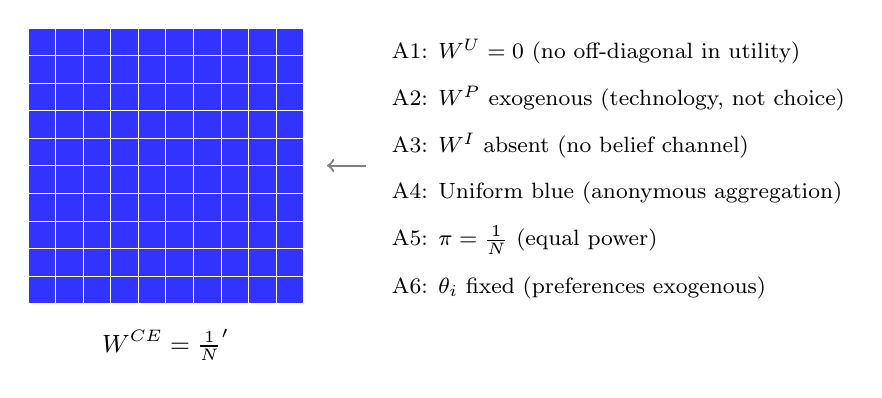
\begin{tikzpicture}[scale=1]
\def\N{10}
\def\s{0.35}
\foreach \i in {1,...,\N} {
  \foreach \j in {1,...,\N} {
    \fill[blue!80!white, draw=white, line width=0.1pt]
      ({(\j-1)*\s}, {(\N-\i)*\s}) rectangle +(\s,\s);
  }
}
\node[below, font=\small\bfseries] at ({5*\s}, -0.2) {$W^{CE} = \frac{1}{N}\ones\ones'$};

\node[font=\footnotesize, anchor=west] at (4.5, 3.2) {A1: $W^U = 0$ (no off-diagonal in utility)};
\node[font=\footnotesize, anchor=west] at (4.5, 2.6) {A2: $W^P$ exogenous (technology, not choice)};
\node[font=\footnotesize, anchor=west] at (4.5, 2.0) {A3: $W^I$ absent (no belief channel)};
\node[font=\footnotesize, anchor=west] at (4.5, 1.4) {A4: Uniform blue (anonymous aggregation)};
\node[font=\footnotesize, anchor=west] at (4.5, 0.8) {A5: $\boldsymbol{\pi} = \frac{1}{N}\ones$ (equal power)};
\node[font=\footnotesize, anchor=west] at (4.5, 0.2) {A6: $\theta_i$ fixed (preferences exogenous)};

\draw[->, thick, gray] (4.3, 1.75) -- (3.8, 1.75);
\end{tikzpicture}
\end{center}
\vspace{-0.5em}
\small The uniform-blue heatmap is the visual signature of all six assumptions holding simultaneously. Every departure from uniform blue --- a bright column, a dark off-diagonal region, a block structure --- is a violation of at least one assumption.
\end{vizpanel}

The six assumptions are not independent. They form a logical hierarchy:

\begin{proposition}[The Hierarchy of Assumptions]\label{ch04:prop:hierarchy}
\begin{enumerate}
\item A1--A3 are about the \textbf{existence} of the three networks. The standard model denies that $W^U$ matters, takes $W^P$ as exogenous, and ignores $W^I$ entirely.
\item A4 is about the \textbf{symmetry} of the market mechanism. Given that $W^U$ and $W^I$ are absent, the remaining interaction (through prices) is assumed to be anonymous and equal.
\item A5 is a \textbf{consequence} of A1--A4: if the only interaction is through the symmetric market, then the composite $W$ is doubly stochastic and $\boldsymbol{\pi} = \frac{1}{N}\ones$.
\item A6 is the \textbf{deepest} assumption: it says the structure cannot change preferences. Without A6, even a correct diagnosis of the other five becomes dynamically unstable --- the preferences used to evaluate welfare are themselves produced by the network.
\end{enumerate}
\end{proposition}

\begin{keyinsight}
The six assumptions can be summarized in one sentence: \textit{the standard model assumes that social structure is irrelevant for economic outcomes.}

$W^U = 0$: social bonds don't affect utility. $W^P$ exogenous: production structure is engineering, not social choice. $W^I$ absent: information doesn't flow through social channels. $W^{\text{market}} = \frac{1}{N}\ones\ones'$: the market treats everyone the same. $\boldsymbol{\pi} = \frac{1}{N}\ones$: nobody has structural power. $\theta$ fixed: the structure doesn't shape who you become.

Structural economics is the systematic relaxation of this sentence.
\end{keyinsight}


%% =====================================================================
\section{The Structural Program}
\label{ch04:sec:program}
%% =====================================================================

Part~II of this book introduces the three networks ($W^U$, $W^P$, $W^I$) as distinct objects, derives power from the Perron eigenvector, and computes the bargaining equilibrium --- relaxing A1, A3, A4, and A5.

Part~III relaxes A6 --- the formation model, where $W^I$ shapes preferences.

Part~IV studies dynamics --- how the networks evolve and reproduce, relaxing A2 (production structure becomes endogenous).

Parts V--VII apply the framework to three scales (global, national, individual), develop measurement tools, and analyze structural change.

\begin{center}
\begin{tabular}{clll}
\toprule
\textbf{Assumption} & \textbf{Standard model} & \textbf{Structural economics} & \textbf{Chapters} \\
\midrule
A1 ($W^U$) & $= 0$ & General $W^U$ & 5, 7, 12 \\
A2 ($W^P$) & Exogenous & Endogenous, policy variable & 3, 13, 15 \\
A3 ($W^I$) & Absent & Drives beliefs and aspirations & 5, 8, 9--12 \\
A4 (Market) & $\frac{1}{N}\ones\ones'$ & Asymmetric, concentrated & 6, 7 \\
A5 (Power) & $\boldsymbol{\pi} = \frac{1}{N}\ones$ & $\boldsymbol{\pi}(W)$, computed & 6, 7, 16--19 \\
A6 (Preferences) & Fixed $\theta$ & $\theta_{t+1} = f(W^I, \theta_t)$ & 9--12 \\
\bottomrule
\end{tabular}
\end{center}

Each row of this table is a chapter (or group of chapters). Each cell is a research program. The table is the book.


%% =====================================================================
\section{How Far Is the Real World from $W^{CE}$?}
\label{ch04:sec:how_far}
%% =====================================================================

A natural question: are we tilting at windmills? How badly do the assumptions fail in practice?

\begin{proposition}[Empirical Departures]\label{ch04:prop:empirical}
For each assumption, we can define a scalar measure of departure and estimate it from data:
\begin{center}
\begin{tabular}{clcc}
\toprule
& \textbf{Departure measure} & \textbf{Data source} & \textbf{Typical value} \\
\midrule
A1 & $\gamma_U \|W^U\|_F$ (externality intensity) & Social surveys & $0.1$--$0.5$ \\
A2 & $\Delta A / A$ (I-O change per decade) & I-O time series & $5$--$20\%$ \\
A3 & $\Var(\pi^I_i)$ (epistemic power concentration) & Media data & $0.01$--$0.10$ \\
A4 & $\Delta(W^{\text{market}})$ (column-sum asymmetry) & Market shares & $0.1$--$0.8$ \\
A5 & $\Var(\pi_i)$ (power asymmetry) & Composite $W$ & $0.001$--$0.05$ \\
A6 & $\Psi$ ratio (formation vs.\ enforcement) & Cohort-year data & $0.5$--$4.0$ \\
\bottomrule
\end{tabular}
\end{center}
\end{proposition}

The departures are not small. In Bolivia's domestic production network, the column-sum asymmetry $\Delta(W^P)$ is approximately 0.4 (Chapter~3). The $\Psi$ ratio for female labor force participation in the US is approximately 2.1 (Chapter~11). The epistemic power concentration of global financial media gives $\Var(\pi^I_i) \approx 0.03$ for a 20-country sample.

The standard model is a useful benchmark --- like Euclidean geometry in a curved universe. But the curvature is measurable, and in development economics it is large.

\begin{vizpanel}{From $W^{CE}$ to the real world: five departures}
\begin{center}
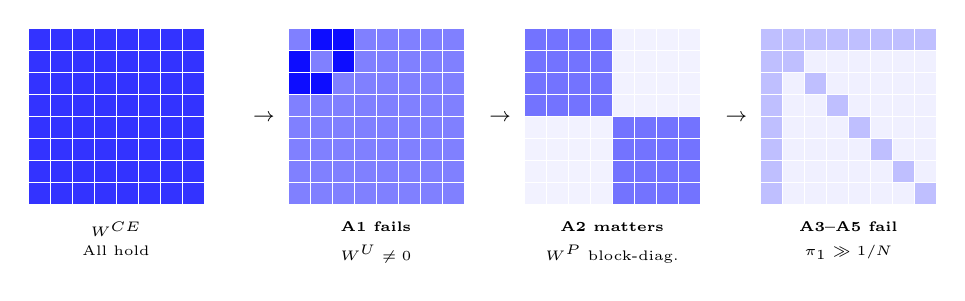
\begin{tikzpicture}[scale=1]
\def\N{8}
\def\s{0.28}

%% 1. W^CE
\foreach \i in {1,...,\N} {
  \foreach \j in {1,...,\N} {
    \fill[blue!80, draw=white, line width=0.08pt]
      ({(\j-1)*\s}, {(\N-\i)*\s}) rectangle +(\s,\s);
  }
}
\node[below, font=\tiny\bfseries] at ({4*\s}, -0.1) {$W^{CE}$};
\node[below, font=\tiny] at ({4*\s}, -0.4) {All hold};

%% Arrow
\node[font=\scriptsize] at (3.0, 1.1) {$\to$};

%% 2. Add utility externalities (cluster)
\begin{scope}[xshift=3.3cm]
\foreach \i in {1,...,\N} {
  \foreach \j in {1,...,\N} {
    \pgfmathparse{(\i<=3 && \j<=3 && \i!=\j) ? 95 : 50}
    \edef\bp{\pgfmathresult}
    \fill[blue!\bp, draw=white, line width=0.08pt]
      ({(\j-1)*\s}, {(\N-\i)*\s}) rectangle +(\s,\s);
  }
}
\node[below, font=\tiny\bfseries] at ({4*\s}, -0.1) {A1 fails};
\node[below, font=\tiny] at ({4*\s}, -0.4) {$W^U \neq 0$};
\end{scope}

\node[font=\scriptsize] at (6.0, 1.1) {$\to$};

%% 3. Block-diagonal production
\begin{scope}[xshift=6.3cm]
\foreach \i in {1,...,\N} {
  \foreach \j in {1,...,\N} {
    \pgfmathparse{(\i<=4 && \j<=4) ? 65 : (\i>4 && \j>4) ? 55 : 5}
    \edef\bp{\pgfmathresult}
    \fill[blue!\bp, draw=white, line width=0.08pt]
      ({(\j-1)*\s}, {(\N-\i)*\s}) rectangle +(\s,\s);
  }
}
\node[below, font=\tiny\bfseries] at ({4*\s}, -0.1) {A2 matters};
\node[below, font=\tiny] at ({4*\s}, -0.4) {$W^P$ block-diag.};
\end{scope}

\node[font=\scriptsize] at (9.0, 1.1) {$\to$};

%% 4. Star W^I
\begin{scope}[xshift=9.3cm]
\foreach \i in {1,...,\N} {
  \foreach \j in {1,...,\N} {
    \pgfmathparse{(\j==1) ? 70 : (\i==1) ? 15 : (\i==\j) ? 25 : 6}
    \edef\bp{\pgfmathresult}
    \fill[blue!\bp, draw=white, line width=0.08pt]
      ({(\j-1)*\s}, {(\N-\i)*\s}) rectangle +(\s,\s);
  }
}
\node[below, font=\tiny\bfseries] at ({4*\s}, -0.1) {A3--A5 fail};
\node[below, font=\tiny] at ({4*\s}, -0.4) {$\pi_1 \gg 1/N$};
\end{scope}
\end{tikzpicture}
\end{center}
\vspace{-0.5em}
\small Progressive departure from the competitive benchmark. Each step adds a structural feature that the standard model assumes away. The real world is on the right --- and further right than the last panel shows.
\end{vizpanel}


%% =====================================================================
\section{Summary}
\label{ch04:sec:summary}
%% =====================================================================

\begin{enumerate}
\item The standard competitive model makes six assumptions, all expressible as properties of the weight matrix: $W^U = 0$, $W^P$ exogenous, $W^I$ absent, $W^{\text{market}} = \frac{1}{N}\ones\ones'$, $\boldsymbol{\pi} = \frac{1}{N}\ones$, and $\theta$ fixed.

\item The assumptions form a hierarchy: A1--A3 deny the existence of three networks; A4 asserts symmetry of the remaining interaction; A5 follows as a consequence; A6 freezes the structure by fixing preferences.

\item Each assumption has a measurable departure: externality intensity, I-O change rates, epistemic power concentration, column-sum asymmetry, power variance, and the $\Psi$ ratio. In developing economies, the departures are large.

\item Structural economics is the systematic relaxation of these six assumptions: Parts II--VII develop general $W^U$, endogenous $W^P$, general $W^I$, asymmetric power, and endogenous preferences.

\item The standard model is not wrong. It is the special case $W = \frac{1}{N}\ones\ones'$ with $\theta$ fixed. This book is the general case.
\end{enumerate}


%% =====================================================================
\section{Exercises}
\label{ch04:sec:exercises}
%% =====================================================================

\begin{enumerate}[label=\textbf{4.\arabic*}, leftmargin=3em]

\item \textbf{Classifying failures.} For each scenario, identify which of A1--A6 is violated and which is the most important:
\begin{enumerate}
\item A landlord and three tenant farmers negotiate sharecropping rates in a village with no outside labor market.
\item A social media platform shows users algorithmically selected content that shifts purchasing behavior.
\item Bolivia's gas revenues are redistributed through transfers, but the gas sector remains an enclave.
\item A girl in Potos\'{i} with a smartphone develops aspirations her mother never had.
\item Two ethnic groups in the same city trade goods but do not intermarry, share schools, or attend the same churches.
\end{enumerate}

\item \textbf{Measuring departure.} For a $3 \times 3$ row-stochastic matrix $W = \begin{pmatrix} 0.5 & 0.3 & 0.2 \\ 0.1 & 0.7 & 0.2 \\ 0.2 & 0.1 & 0.7 \end{pmatrix}$:
\begin{enumerate}
\item Compute column sums. Is $W$ doubly stochastic?
\item Compute $\Delta(W) = \|\ones'W - \ones'\|_2$.
\item Compute the Perron eigenvector $\boldsymbol{\pi}$ and $\Var(\pi_i)$.
\item If this were Bolivia's composite $W$ (with $N = 3$ sectors), which assumption is most severely violated?
\end{enumerate}

\item \textbf{The hierarchy in action.} Construct a $4 \times 4$ economy where:
\begin{enumerate}
\item A1 fails but A4 holds (utility externalities exist, but the market interaction is still symmetric). Is $\boldsymbol{\pi}$ uniform? (Hint: the composite $W$ includes $W^U$.)
\item A4 fails but A1 holds (market power exists, no utility externalities). Is $\boldsymbol{\pi}$ uniform?
\item Both A1 and A4 fail simultaneously. Compute $\boldsymbol{\pi}$. Is the welfare loss larger than the sum of the individual losses? (This tests whether the interaction term $L_{\text{int}}$ is positive.)
\end{enumerate}

\item \textbf{Bolivia's six assumptions.} Using the two-sector Bolivia model from Chapter~3 ($W^P$ with Gas and Traditional):
\begin{enumerate}
\item Assess each of A1--A6 for Bolivia. Which hold approximately? Which fail clearly?
\item For each failing assumption, estimate the departure measure from publicly available data (INE, CEPAL).
\item Rank the six departures from largest to smallest. Which structural feature of Bolivia is the most severe deviation from the competitive benchmark?
\end{enumerate}

\item \textbf{Sunkel's five processes.} Sunkel (1971) argued that development, underdevelopment, dependency, marginalization, and spatial inequality are ``diverse manifestations of a single process.'' Formalize this: define each of the five processes as a property of the weight matrix $W$ or its components ($W^U$, $W^P$, $W^I$). What is the ``single process'' in matrix terms?

\item \textbf{A6 is the deepest.} Consider two economists:
\begin{enumerate}
\item Economist A relaxes A1--A5 but keeps A6 (preferences are fixed). She finds the optimal policy: a transfer $T^*$ that maximizes welfare given the structural power $\boldsymbol{\pi}(W)$.
\item Economist B relaxes all six, including A6. She finds that the policy changes $W^I$, which changes $\theta$, which changes the welfare function itself.
\item Show that Economist A's policy can be welfare-\textit{reducing} under Economist B's model. (Hint: the transfer may reinforce the information structure that produces low aspirations.)
\item What does this imply about the ``growth first, redistribute later'' consensus?
\end{enumerate}

\item \textbf{The spectral gap of the assumptions.} For $N = 8$, construct a sequence of matrices $W^{(k)}$ for $k = 0, 1, \ldots, 5$ where $W^{(0)} = \frac{1}{8}\ones\ones'$ and each successive matrix adds one structural feature (a cluster in $W^U$, a block in $W^P$, a hub in $W^I$, etc.). Compute $\Gamma^{(k)}$ and $L^{(k)}_{\text{power}}$ for each. Plot both as functions of $k$. Does the welfare loss grow linearly, convexly, or concavely in the number of structural features?

\end{enumerate}


%% =====================================================================
\newpage
\section*{Mathematical Appendix}
\addcontentsline{toc}{section}{Mathematical Appendix}
%% =====================================================================

\subsection*{Appendix 4A: Composite Matrices and Their Perron Eigenvectors}
\addcontentsline{toc}{subsection}{Appendix 4A: Composite Matrices}
\label{ch04:app:composite}

\paragraph{The composite.} Given three nonnegative matrices $W^U, W^P, W^I$ (each $N \times N$) and weights $\alpha_U + \alpha_P + \alpha_I = 1$ with $\alpha_k \geq 0$:
\begin{equation}
W = \alpha_U W^U + \alpha_P W^P + \alpha_I W^I.
\end{equation}

If each component is row-stochastic, so is $W$: $W\ones = \alpha_U W^U\ones + \alpha_P W^P\ones + \alpha_I W^I\ones = \alpha_U\ones + \alpha_P\ones + \alpha_I\ones = \ones$.

\paragraph{Perron eigenvector of the composite.} In general, $\boldsymbol{\pi}(W)$ is NOT a convex combination of $\boldsymbol{\pi}(W^U)$, $\boldsymbol{\pi}(W^P)$, $\boldsymbol{\pi}(W^I)$. The eigenvectors of a sum of matrices are not the sums of the eigenvectors. This is a nonlinearity that makes the composite power vector genuinely different from any single-network power vector.

\paragraph{Special cases.} If all three components have the same eigenvector ($\boldsymbol{\pi}^U = \boldsymbol{\pi}^P = \boldsymbol{\pi}^I = \boldsymbol{\pi}$), then $\boldsymbol{\pi}(W) = \boldsymbol{\pi}$ --- the composite inherits the common power structure. This is the ``aligned networks'' case from Chapter~5: all three networks agree on who is powerful. In this case, power is reinforced across channels.

If the components have different eigenvectors, the composite $\boldsymbol{\pi}(W)$ is a nonlinear blend that depends on the $\alpha_k$ weights. Changing $\alpha_P$ (the importance of production linkages) relative to $\alpha_I$ (the importance of information) can shift $\boldsymbol{\pi}$ discontinuously when the leading eigenvectors of $W^P$ and $W^I$ point in very different directions. This is a structural phase transition: the economy's power structure flips when one network channel comes to dominate.

\paragraph{Computing $\boldsymbol{\pi}(W)$.} Form $W = \alpha_U W^U + \alpha_P W^P + \alpha_I W^I$, then apply power iteration (Appendix~6A).


%% =====================================================================
\subsection*{Structuralist Case Study: Sunkel and Paz's Systematic Critique}
\addcontentsline{toc}{subsection}{Structuralist Case Study: Sunkel and Paz (1970)}
%% =====================================================================

In 1970, Osvaldo Sunkel and Pedro Paz published \textit{El subdesarrollo latinoamericano y la teor\'{i}a del desarrollo} through ILPES/Siglo XXI --- a 385-page treatise that remains the most comprehensive systematic critique of orthodox development theory from the structuralist perspective. Where Prebisch (1949) was a manifesto and Furtado (1961) was a theoretical essay, Sunkel and Paz was a textbook: methodical, exhaustive, and organized as a point-by-point examination of what mainstream economics assumes and why those assumptions fail in the periphery.

Their argument maps directly onto the six assumptions of this chapter.

\textbf{Part 1: Mainstream theory assumes a closed, self-contained economy.} Sunkel and Paz began by noting that the neoclassical model analyzes an economy in isolation --- abstracting from its insertion in the global system. They argued that this is not an innocuous simplification but a fundamental distortion: the peripheral economy's structure is shaped by its relationship to the center. In our notation: the standard model treats $W^P$ as a domestic object, ignoring the global production network in which the domestic matrix is embedded. The domestic $W^P$ is not independent of the global $W^P$ --- the off-diagonal entries linking the domestic economy to the world are among the most important entries in the matrix.

\textbf{Part 2: Five processes, one process.} The book's most original contribution was the claim that development, underdevelopment, dependency, marginalization, and spatial inequality are not five separate phenomena but ``diverse manifestations of a single process'' --- the simultaneous transnational integration and national disintegration produced by global capitalism. In matrix terms: the global weight matrix $W_{\text{global}}$ is being rewired in a way that increases cross-country connectivity among elite nodes (transnational integration) while decreasing within-country connectivity between elite and non-elite nodes (national disintegration). The five ``processes'' are five observables of one matrix transformation.

\textbf{Part 3: The theory is part of the structure.} Sunkel and Paz argued --- anticipating Quijano by three decades --- that the economic theories taught at the center and exported to the periphery are not neutral analytical tools but products of the center's structural position. The theory of comparative advantage, the Heckscher-Ohlin model, the welfare theorems --- these are theorems about $W = \frac{1}{N}\ones\ones'$, which is the center's idealization of a world that serves the center's interests. Teaching these theorems in La Paz without noting that they assume a specific $W$ is an act of epistemic power: it naturalizes the assumption that makes the welfare theorems hold, thereby legitimating the structure that the theorems describe.

\begin{center}
\begin{tabularx}{\textwidth}{LLL}
\toprule
\textbf{Sunkel \& Paz's argument} & \textbf{This chapter's assumption} & \textbf{Formal object} \\
\midrule
Economy not self-contained & A2: $W^P$ treated as domestic & Global embedding of $W^P$ \\
Five processes, one process & A1--A5 fail simultaneously & $W \neq \frac{1}{N}\ones\ones'$, all channels \\
National disintegration & A4: market not symmetric & Block-diagonal domestic $W$ \\
Transnational integration & A2: $W^P$ changes endogenously & Elite cross-border linkages \\
Theory is part of structure & A6: preferences exogenous & $W^I$ shapes beliefs about theory \\
\bottomrule
\end{tabularx}
\end{center}

Sunkel and Paz's book is the structuralist critique organized as a textbook. This chapter is the same critique organized as a table of matrix properties. The mathematics adds precision; the diagnosis was always theirs.


%% =====================================================================
\subsection*{Further Reading}
\addcontentsline{toc}{subsection}{Further Reading}
%% =====================================================================

\textbf{The welfare theorems and their assumptions:} MWG (1995), Chapter~16; Debreu (1959); Arrow (1951). For the assumptions' failure in developing economies: Stiglitz (1989), ``Markets, Market Failures, and Development,'' \textit{AER P\&P}.

\textbf{Endogenous production networks:} Acemoglu et al.\ (2012); Baqaee and Farhi (2019); Hidalgo et al.\ (2007), ``The Product Space Conditions the Development of Nations,'' \textit{Science}.

\textbf{Information networks and belief dynamics:} DeGroot (1974); Golub and Jackson (2010); Acemoglu et al.\ (2011), ``Bayesian Learning in Social Networks,'' \textit{ReStud}.

\textbf{Endogenous preferences:} Bowles (1998), ``Endogenous Preferences: The Cultural Consequences of Markets and Other Economic Institutions,'' \textit{JEL}; Bisin and Verdier (2001), ``The Economics of Cultural Transmission and the Dynamics of Preferences,'' \textit{JET}.

\textbf{The structuralist critique:} Sunkel and Paz (1970), \textit{El subdesarrollo latinoamericano y la teor\'{i}a del desarrollo}, M\'{e}xico: Siglo XXI / ILPES (the definitive systematic treatment; the full text in Spanish is available through CEPAL's digital repository). Sunkel (1971), ``Capitalismo transnacional y desintegraci\'{o}n nacional en Am\'{e}rica Latina,'' \textit{Estudios Internacionales} 4(16), pp.~3--61.

\end{document}
